% Este trabalho está licenciado sob a Licença Atribuição-CompartilhaIgual 4.0 Internacional Creative Commons. Para visualizar uma cópia desta licença, visite http://creativecommons.org/licenses/by-sa/4.0/deed.pt_BR ou mande uma carta para Creative Commons, PO Box 1866, Mountain View, CA 94042, USA.

\chapter{Linguagem de Programação}\label{cap_lingua}
\thispagestyle{fancy}

\section{Computador}\label{cap_lim_sec_computador}

\begin{flushright}
  [YouTube] | [Vídeo] | [Áudio] | [Contatar]
\end{flushright}

Um computador\footnote{Consulte \href{https://pt.wikipedia.org/wiki/Computador}{Wikipédia: Computador} para uma introdução sobre a história e outras questões sobre computadores.} é um \emph{sistema computacional} de elementos físicos (\emph{hardware}) e elementos lógicos (\emph{software}).

O \emph{hardware} são suas partes mecânicas, elétricas e eletrônicas como: fonte de energia, teclado, mouse/painel tátil, monitor/tela, dispositivos de armazenagem de dados (HDD, {\it hard disk drive}; SSD, {\it solid-state drive}; RAM, {\it random-access memory}; etc.), dispositivos de processamento (CPU, {\it central processing unit}, GPU, {\it graphics processing unit}), conectores de dispositivos externos (microfone, caixa de som, fone de ouvido, USB, etc.), placa mãe, etc..

O \emph{software} é toda a informação processada pelo computador, qualquer código executado e qualquer dado usado nas computações.

\begin{figure}[H]
  \centering
  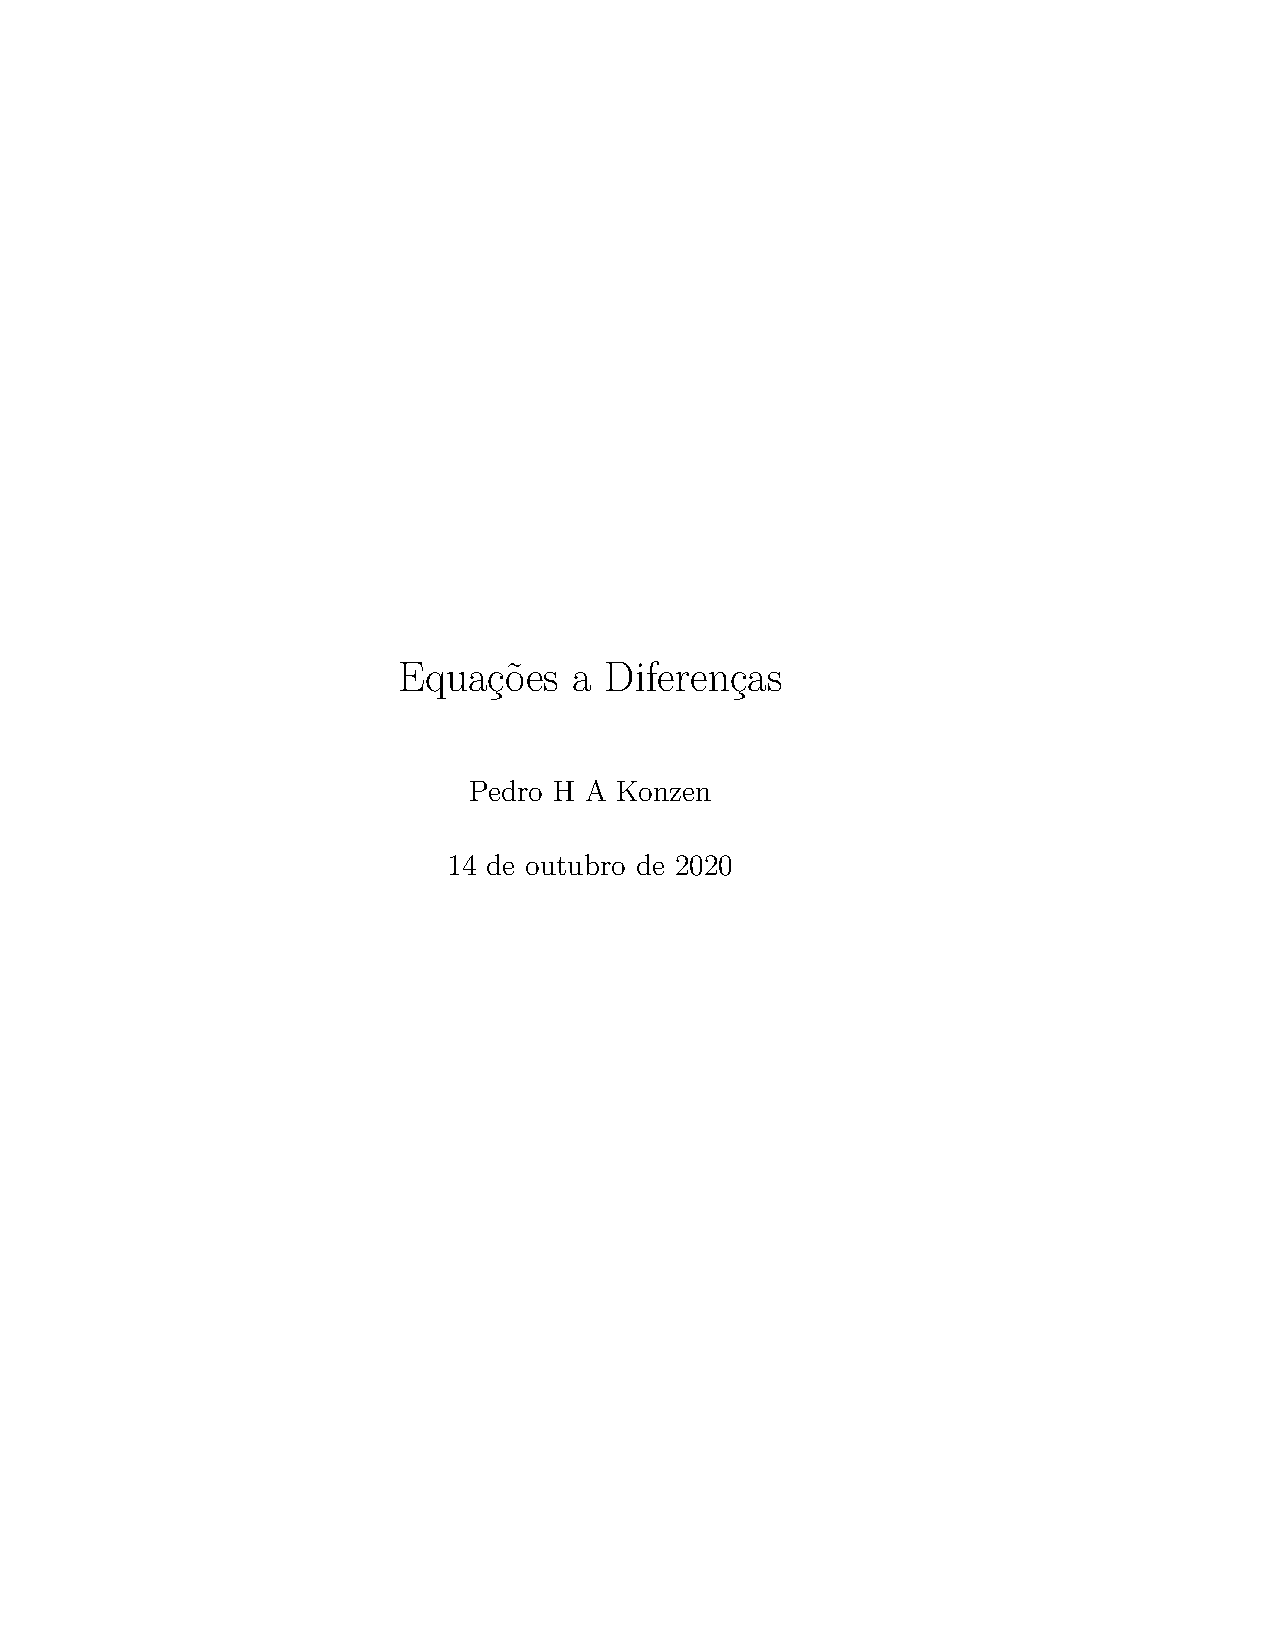
\includegraphics[width=\textwidth]{./cap_lingua/dados/fig_vonNeumann/main}
  \caption[Arquitetura de von Neumann]{Arquitetura de computador de von Neumann.}
  \label{cap_lim_sec_computador:fig:arqVonNeumann}
\end{figure}

Os computadores que comumente utilizamos seguem a arquitetura de John von Neumann\footnote{John von Neumann, 1903 - 1957, matemático húngaro, naturalizado estadunidense. Fonte: \href{https://pt.wikipedia.org/wiki/John_von_Neumann}{Wikipédia}.}, que consiste em dispositivo(s) de entrada de dados, unidade(s) de processamento, unidade(s) de memória e dispositivo(s) de saída de dados (Figura~\ref{cap_lim_sec_computador:fig:arqVonNeumann}).

\emconstrucao

\subsection{Exercícios Resolvidos}

\emconstrucao

\subsection{Exercícios}

\emconstrucao
